\chapter{Evaluatiion}

% Requirements
% * Functional
% * Non-functional
%
% Algorithm
% * Gleichverteilt
% * Umfrage
%
% Implementation
% * scaling
% * ldap connections sind ne bitch
%
% Conclusion

\section{Implementation}
\subsection{Scalability}
A software system has to be able to scale according to the number of its users in order to be future-proof, as the current trend to dynamically scalable cloud solutions and server-less web architecture approaches highlights. There are two concepts or preparing an application for an higher workload: vertical scaling and horizontal scaling. Vertical scaling is done by providing more resources, e.g. Memory and CPU power, to the machines running the applicaions. Horziontal scaling, however, means setting up more machines providing the same service, so that workload can be distributed between them \cite{hvscale}. In contrast to vertical scaling, horizontal scaling has vital advantages: the application will be more robust since the crashing of one machine can be compensated by others \cite{fedi}, the capacity of the system can, theoretically, be unlimited, and it is cheaper, because instances can be created dynamically if needed and then be destroyed in times of low workload, whereas the resources given to a machine that has been scaled vertically will remain unused.

\begin{figure}[!htp]
    \centering
    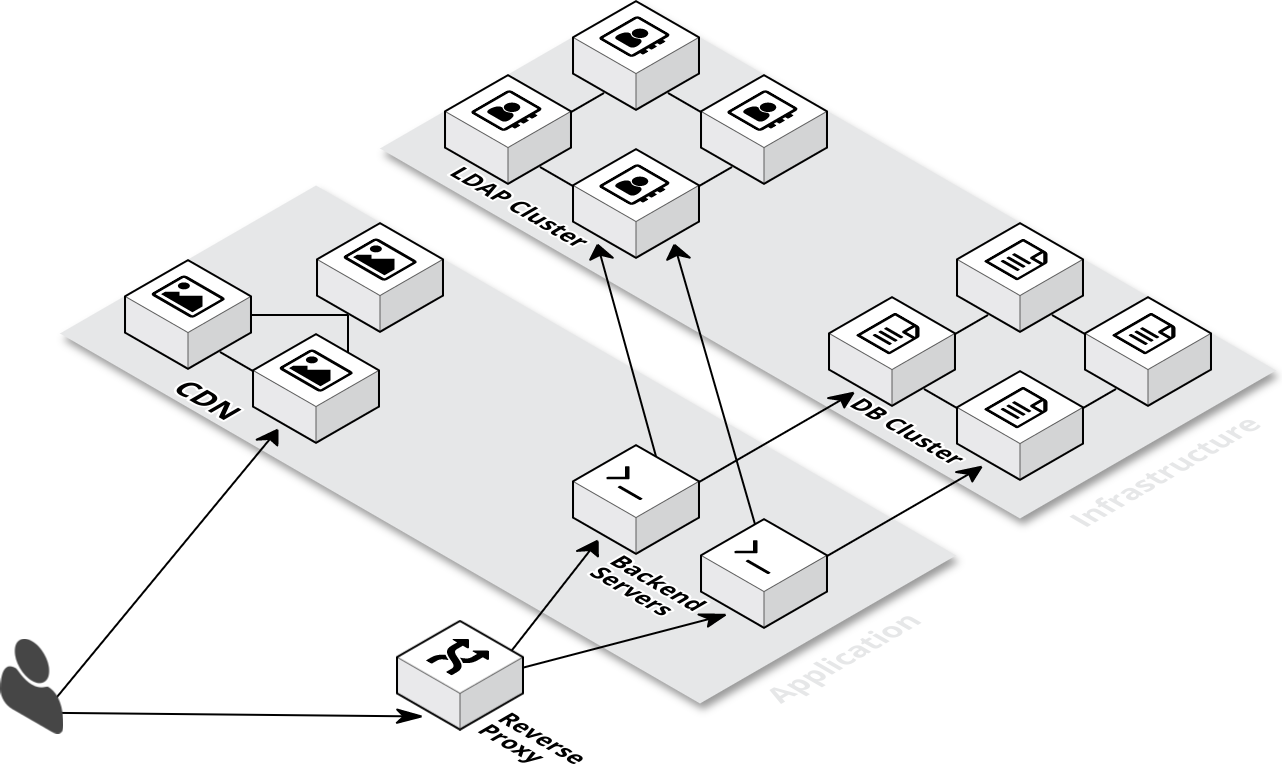
\includegraphics[width=0.75\textwidth]{images/system_architecture_scaled.png}
    \caption[System Architecture (scaled up)]{A possible approach to scale the system using multiple backend servers, a CDN, and multiple clustered database and ldap servers. Created with \textit{https://cloudcraft.co}.}
    \label{scaleup}
\end{figure}

\subsubsection{MongoDB}
MongoDB is meant to be scaled horizontally and supports the adding of new instances to a running cluster of databases out-of-the-box \cite[p. 19]{MongoGuide}. So, new machines running the database as a cluster will be created, if needed. As shown in \ref{scaleup}, the backend servers can be connected to any of the database servers in order to request data. If the demanded document is not found on the instance the backend is connected to, MongoDB will handle the lookup in the cluster; to the application, the cluster is completely transparent and appear as if it was one machine.

\subsubsection{LDAP}
The LDAP servers\footnote{SinnerSchrader is running \textit{OpenLDAP} (http://www.openldap.org)} can also be run as a cluster in order to improve response times and prevent data loss by replicating the stored information \cite{ldapscale}. In fact, the LDAP is currently being provided by six servers that represent the service. As illustrated in \ref{scaleup}, the backend servers can connect to any of the LDAP servers; the data replication and synchronization is handled transparently.

\subsubsection{Static Content}
The static content files like HTML, CSS and JS files, that altogether represent the frontend, are
served by the reverse proxy web server. In the event of an increasing number of requests that cannot be handled by the single server, a \textit{Content Delivery Network} (CDN) could be deployed. A CDN is a network of webservers that provide static content and large files. The reverse proxy would redirect the URLs for those files, so that the users' browsers will connect directly to said network in order to retrieve the assets.

\subsubsection{Backend}
The backend application itself does not save any data on the machine it is running on, but connects a database server (see \ref{impl:be}). As a result, any number of backend instances can be set up. In contrast to the other services, the backend servers do not have to synchronize. In order to receive HTTP requests, the reverse proxy must be configured so that it redirects API calls to the backend servers. This is called \textit{load balancing} and is supported by many modern web servers such as \textit{nginx}, \textit{Apache} and \textit{Tomcat}.

\subsection{Conclusion}
In theory, the application should be able to scale according to the number of its users. Practically, only the running of multiple backend and LDAP servers has been tested successfully. Running multiple database instances has not been tested; since MongoDB has been designed to be horizontally scalable and comes to use in various companies like
\textit{Github}\footnote{https://www.mongodb.com/presentations/mongosv-2012/mongodb-analytics-github},
\textit{eBay}\footnote{https://www.mongodb.com/presentations/mongodb-ebay}, and
\textit{Otto}\footnote{https://www.mongodb.com/industries/retail}, it can be assumed that this can be done successfully for this application, too.
Deploying a CDN that serves the static content has not been evaluated, as the implementation of the frontend was not part of this thesis, but has been worked on by \cite{strecker}. 
